\graphicspath{{etatArtImages/}}
\chapter{Etat de l'art}


Comme nous l’avons vu, comprendre le langage naturel de l’utilisateur nécessite le système NLP décomposé en NLU pour comprendre et NLG pour répondre.
\vspace{1em}

 Mais, comment peut-on programmer ce dialogue ?
	Il existe plusieurs techniques. Nous allons en aborder trois qui sont liées aux dialogues homme-machine. La première fera référence à de l’algorithme sur le TAL (Traitement automatique des langues) en python. La deuxième à L’Artificial Intelligence Markup Language(AIML) qui est un langage hérité de XML et utilisé pour les tout premiers chatbots. Et le troisième, le dialogue géré avec des intents qui commence à émerger notamment utilisé pour Cortana.
\vspace{1em}
	
	Dans un second temps, nous regarderons ce qu’apporte chaque solution. Puis, nous évaluerons leurs impacts dans le paramétrage d’un chatbot.


\section{Etudes et expérimentation sur le TAL via NLTK}


\subsection{TAL}


Le traitement automatique des langues est une discipline qui combine linguistique, informatique et formalisme.  Le but de cette discipline est de développer des logiciels pour traiter le langage naturel par ordinateur de façon automatique.
\vspace{1em}

	L’objectif est de donner aux ordinateurs les capacités linguistiques d’un être humain. Elle existe depuis les années 50 comme le début de l’IA avec les traductions automatiques.
	\vspace{1em}
	
	Pour les niveaux de traitements, il faut se référer aux chapitres concept sur le natural language understanding qui traite des différentes analyses du langage.
	\vspace{1em}
	
	Dans un entretien avec un chercheur de Paris X, Marcel Cori explique les techniques mises en œuvre :
	\vspace{1em}
	
« C’est une recherche en linguistique et une recherche en informatique, puisqu’il s’agit de définir des modèles et des algorithmes sur ces modèles de données langagières. ». \cite{ref8}
\vspace{1em}

Pour parler du TAL et des algorithmes, nous allons nous intéresser du côté du langage python et d’une librairie qui existe pour appliquer le TAL, qui est le Python Natural Language ToolKit (NLTK).


\subsection{NLTK}

Le NLTK est un ensemble de modules python qui implémente des algorithmes pour le TAL. Il permet de faire un traitement des expressions régulières qui sera le cœur de cette méthode pour extraire les mots d’une phrase. Une fois les mots extraits, ils sont étiquetés en suivant des règles pour les catégoriser puis, les analyser en arbre syntaxique.

\subsubsection{Segmentation}

La segmentation du texte consiste à découper en “mots ”ou “segments”. Elle est obligatoire pour commencer toutes applications TAL. Elle détermine les unités de base à partir desquelles ces applications pourront travailler.
\vspace{1em}

Dans la libraire on a la fonction  qui prend en entrée une chaine de caractères et une expression régulière et renvoie en sortie, la liste des chaines qui matchent cette expression régulière.
\vspace{1em}

Une expression régulière spécifie un pattern de caractères, ce pattern sert à identifier certains types de chaines.


\subsubsection{Etiquetage}

Après segmentation on associe à chaque mot une étiquette pour l’identifier.
\vspace{1em}

On a 8 grandes catégories : nom, verbe, pronom, préposition, adverbe, conjonction, adjectif et article. 
\vspace{1em}

Avec d’autres modèles comme Penn Treebank, on a 45 étiquettes ou encore Susanne avec 353 étiquettes.
\vspace{1em}

Modèle Penn Treebank : \cite{ref9}
\vspace{1em}


\begin{figure}[H]
	\centering
		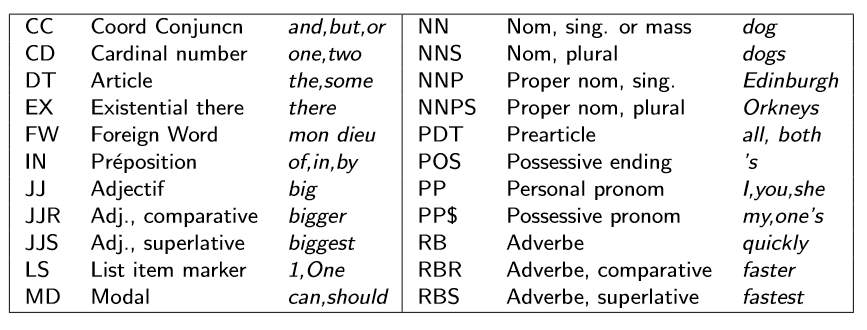
\includegraphics[width = \textwidth]{modele1.png}
	\caption{Modèle1 Penn Treebank}
	\label{fig:Modèle1 Penn Treebank}
\end{figure}

\begin{figure}[H]
	\centering
		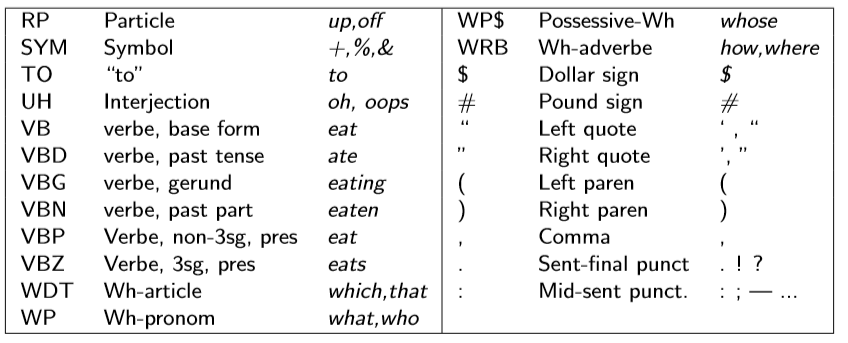
\includegraphics[width = \textwidth]{modele2.png}
	\caption{Modèle2 Penn Treebank}
	\label{fig:Modèle2 Penn Treebank}
\end{figure}

\subsubsection{Analyse}

Après l’étiquetage, on fait une analyse syntaxique ce qui donne, un arbre en sortie après décomposition de la phrase.
\vspace{1em}

On peut retrouver un exemple (figure \ref{fig:Analyse syntaxique})qui explique le TAL \cite{ref10} avec une phrase « Jean a mangé des pommes », le résultat est le suivant de l’analyse est le suivant :
\vspace{1em}

U1 : Jean
U2 : a mangé
U3 : des
U4 : pommes

\begin{figure}[H]
	\centering
		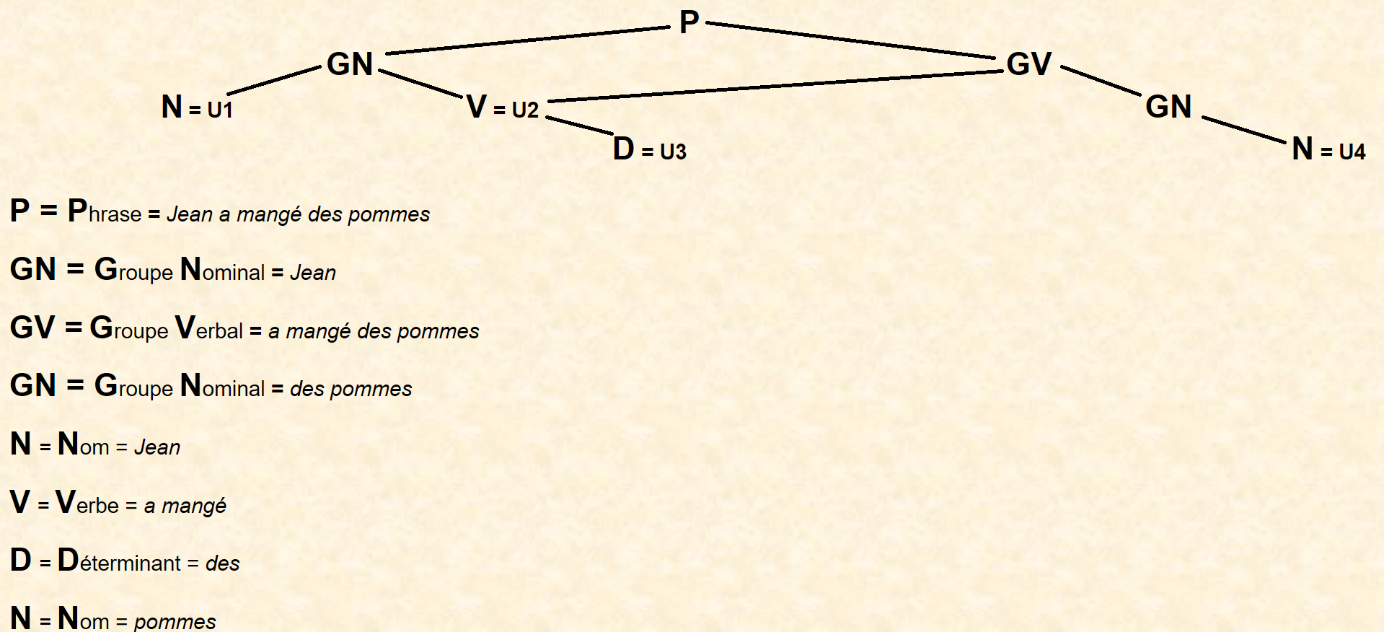
\includegraphics[width = \textwidth]{analyseSyntaxique.png}
	\caption{Analyse syntaxique}
	\label{fig:Analyse syntaxique}
\end{figure}

\section{Etudes et expérimentation sur l'AIML}

Le robot baptisé A.L.I.C.E créé en $1995$ utilise l’AIML qui se sert des fichiers dont le contenu est conforme aux normes XML. Tout fichier AIML donne une liste de schémas auxquels une phrase peut correspondre et celle-ci propose une autre liste de réponses possibles à cette dernière.
\vspace{1em}

Exemple simplifié de fichier AIML en français \cite{ref11}:
\vspace{1em}

<pattern>Raconte-moi une blague </pattern>
<template>Une poule rencontre une autre poule. - Tu viens, lui dit-elle, on va prendre un ver ? </template>
\vspace{1em}

Ainsi, si l’utilisateur demande précisément « Raconte-moi une blague » au chatbot, la réponse renvoyée sera « Une poule rencontre une autre poule. - Tu viens, lui dit-elle, on va prendre un ver ? Il est possible d’ajouter plusieurs réponses (template) pour un même schéma (pattern). 

\subsection{Catégories}

Alice était ainsi le premier chatbot à coupler l’AIML avec une base connaissance. En effet, après la phrase de l’utilisateur, le système matchait un pattern avec la base connaissance pour ensuite fournir une réponse. \cite{ref12}
\vspace{1em}

Chaque catégorie est une partie de la base de connaissance que contient le chatbot.
\vspace{1em}

Exemple simplifié de fichier AIML en français avec plusieurs catégories \cite{ref11} :
\vspace{1em}

<category><pattern>COMMENT CA VA ?</pattern><template>bien et vous? </template></category>
\vspace{0.5em}

<category><pattern>QUEL EST TON NOM ?</pattern><template>je m’appelle Alice</template></category>

\subsection{Récursivité}

AIML implémente la récursivité avec la balise <srai> ce qui permet d’interpréter plus d’entrées de la part de l’utilisateur, nous allons voir quelques exemples pour mieux comprendre.

\subsubsection{Réduction symbolique}

La réduction symbolique se réfère au processus de simplifier des formes grammaticales complexes en formes plus simples. Par exemple, nous avons tendance à préférer des modèles comme "QUI EST SOCRATES" aux comme "VOUS SAVEZ QUI SOCRATES EST" en stockant des informations biographiques sur Socrates.
\vspace{1em}

<category><pattern>WHO IS ALAN TURING ?</pattern><template>Alan Turing was a British mathematician, cryptographer, and computer scientist often credited as the founder of modern Computer Science. </template></category>
\vspace{0.5em}

<category><pattern>WHO IS ALBERT SABIN ?</pattern><template>Albert Sabin was the researcher who developedthe vaccine that is the main defense against polio. </template></category>
\vspace{0.5em}

<category><pattern>DO YOU KNOW WHO * IS ?</pattern><template><srai> WHO IS <star/></srai></template></category>
\vspace{1em}

	L’expression étoile ‘*’ sera reprise dans la balise star qui fera ensuite référence à Alan Turing ou Albert Sabin que l’on peut représenter (figure \ref{fig:Réduction symbolique AIML}) dans les étapes E et F.
	\vspace{1em}
	
	\begin{figure}[H]
	\centering
		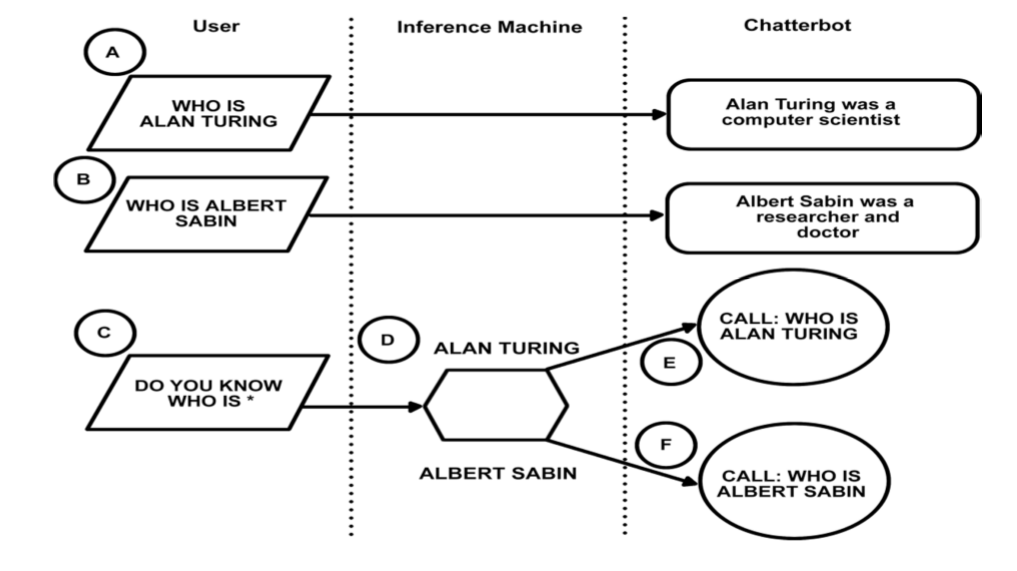
\includegraphics[width = \textwidth]{aiml1.png}
	\caption{Réduction symbolique AIML}
	\label{fig:Réduction symbolique AIML}
\end{figure}

\subsubsection{Diviser pour conquérir}


Une phrase peut être sous divisée en plusieurs sous-phrases. Par exemple, on peut dire bye ou bien bye suivi de ce que l’on veut.
\vspace{1em}

En prenant cet exemple, on a le fichier ci-dessous :
\vspace{1em}

<category><pattern> BYE </pattern><template> Goodbye friend! </template></category>
\vspace{0.1em}

<category><pattern> BYE * </pattern><template><srai> BYE </srai></template></category>
\vspace{1em}

	Dans la deuxième catégorie, si on a bye avec un ou plusieurs mots qui le précèdent alors on appellera le pattern BYE (figure \ref{fig:Diviser pour conquérir AIML}).
\vspace{1em}

\begin{figure}[H]
	\centering
		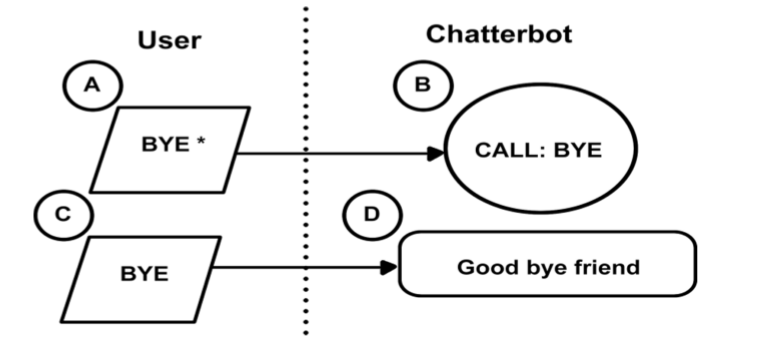
\includegraphics[width = \textwidth]{aiml2.png}
	\caption{Diviser pour conquérir AIML}
	\label{fig:Diviser pour conquérir AIML}
\end{figure}

\subsubsection{Synonyme}

En AIML, on ne peut avoir qu’un pattern par catégorie ;  du coup, on met en place des synonymes qui font référence à un mot.
\vspace{1em}

Exemple d’un fichier avec des synonymes :
\vspace{1em}

<category>
\vspace{0.1em}

<pattern>HELLO</pattern>
\vspace{0.1em}

< template>Hi there!</template>
\vspace{0.1em}

< /category>
\vspace{0.1em}

<category>
\vspace{0.1em}

< pattern>HI</pattern>
\vspace{0.1em}

< template><srai>HELLO</srai></template>
\vspace{0.1em}

< /category>
\vspace{0.1em}

<category>
\vspace{0.1em}
< pattern>HI THERE</pattern>
\vspace{0.1em}

< template><srai>HELLO</srai></template>
\vspace{0.1em}

< /category>
\vspace{1em}

	Il existe encore d’autres balises et principes liés à l’AIML mais l’essentiel a été présenté, le principe étant basé sur des patterns de reconnaissance du message de l’utilisateur.
\vspace{1em}

	Dans une explication sur le principe de l’AIML, il est considéré que lorsque l’on prend la grammaire et la sémantique, le nombre de choses qu’une personne peut finalement dire n’est pas si grande.
	\vspace{1em}
	
	Dans un livre de Steven Pinker, il dit la chose suivante :"Say you have ten choices for the first word to begin a sentence, ten choices for the second word (yielding 100 two-word beginnings), ten choices for the third word (yielding a thousand three-word beginnings), and so on. (Ten is in fact the approximate geometric mean of the number of word choices available at each point in assembling a grammatical and sensible sentence). \cite{ref13}

\section{Etudes et expérimentation sur les intents}

Les derniers chatbots utilisent le modèle sur les intents qui identifie l’intention d’un utilisateur selon son énoncé pour déclencher une action possible en prenant des entités ou non comme paramètres.
\vspace{1em}

	Nous allons expliquer les termes importants puis expliquer avec un exemple issu d’un ouvrage.
\vspace{1em}

Les Intents (intentions) : il s’agit de la fonction que l’application exécute quand l’utilisateur dit quelque chose. Il existe différentes manières de demander la même chose, une intent peut être déclenchée par différents énoncés. Par exemple, “Je veux écouter une chanson de Rihanna” ou “Écouter Rihanna ” devrait lancer une musique de l’artiste Rihanna.
\vspace{1em}

Les Entités : elles représentent un concept. Dans l’exemple précédent sur la musique, Rihanna est une entité qui aurait pu être n’importe quelle autre artiste avec toujours la même fonction, celle d’écouter une musique.
\vspace{1em}

Les Utterances (énoncés) : ce seront tous les énoncés type liés à un intent. Plus on gère de cas possibles et plus le chatbot est susceptible de comprendre à quel intent l’utterance fait référence,  on peut alors parler de machine learning.
\vspace{1em}


\subsection{Exemple d’intent}

Dans l’ouvrage \cite{ref14}, l’explication sur le modèle d’intent se base sur Cortana qui utilise une centaine d’intents avec 25M d’utterances. Dans la partie du livre où il existe ce modèle, il prend pour exemple la phrase suivante « Am I free today at noon ? » (Suis-je libre aujourd’hui à midi ?) en demandant à un chatbot de regarder son calendrier.
\vspace{1em}

	Dans cette question qui est une uttérance de type : « Am I entityat entity ? » le système va faire référence à la fonction read From Calendar avec les entités free today et noon ce qui donne le schéma suivant :
	\vspace{1em}
	
	\begin{figure}[H]
	\centering
		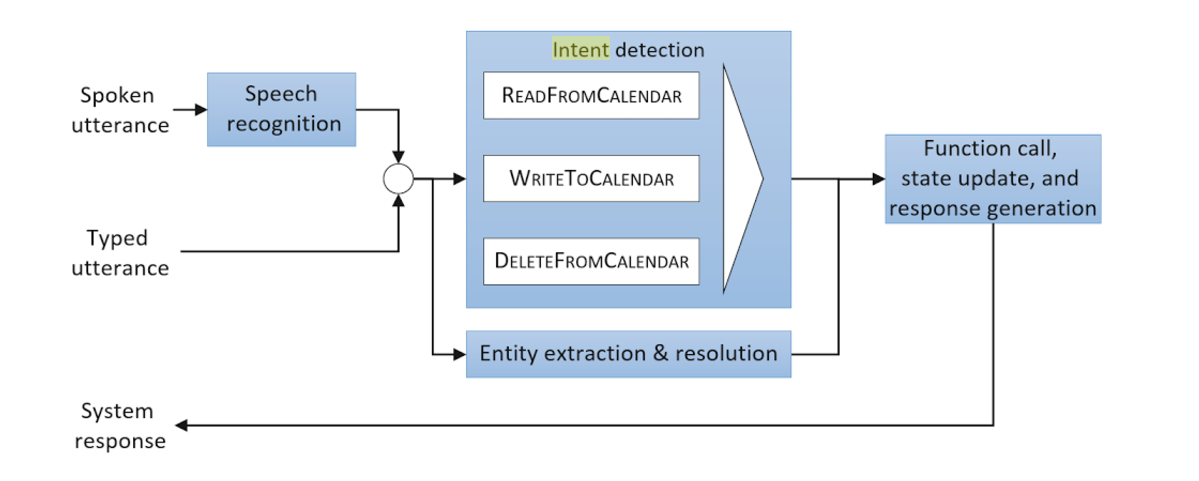
\includegraphics[width = \textwidth]{appelIntent.png}
	\caption{Système d'appel d'intent}
	\label{fig:Système d'appel d'intent}
\end{figure}
	
	
\subsection{Modèle}

Le modèle d’intent est expliqué par le nombre d’utterances permettant de prédéfinir un intent. Un modèle mathématique a été réalisé pour formaliser ce principe. Il a été modélisé par Wang YY, Deng L et Acero A \cite{ref15} et Tur G, Mori RD\cite{ref15} : “Intent i is a model of the form Pi(y|x), where x are the words in the utterance and y is a binary variable where y = 1 indicates that the intent is present in the utterance and y = 0 indicates not. 
\vspace{1em}

For a given utterance x a set of intents P, the most likely intenti* can be selected as :” \cite{ref12} page 3-4
\vspace{1em}


\begin{figure}[H]
	\centering
		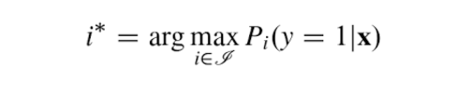
\includegraphics[width = 0.5 \textwidth]{formule.png}
	\caption{Modèle mathématique des intents}
	\label{fig:Modèle mathématique des intents}
\end{figure}
\vspace{1em}

Ainsi, on atteint la valeur maximale de i si l’intent est présent dans l’utterance et qu’il y a le moins de mots possibles avec un modèle.

\subsection{Utilisation du modèle}


Pour comprendre comment des technologies utilisent le modèle d’intent, nous prendrons comme référent la start-up française recast.ai \cite{ref17} qui explique très bien et facilement la manière de créer un chatbot en suivant ce modèle. Il faut savoir que les principes qui seront évoqués sont repris par d’autres sociétés et que  ce sera donc à titre d’exemple.
\vspace{1em}

	Il y a quatre étapes pour créer un chatbot : l’apprentissage, la construction de la logique, l’exécution/déploiement et l’entraînement.


\subsubsection{Apprendre}


A la création d’un chatbot évidemment, il y a un nom à donner puis le ou les langues qui vont être comprises.
\vspace{1em}

	Ensuite, on commence à mettre en place des intents qui vont définir des actions réalisables par le chatbot. Les intents généralement en place sont greetings pour bonjour, hello, etc comme utterance et none lorsque le message ne correspond à aucun intent avec un message type : je ne comprends pas.
	\vspace{1em}

	Quand un intent est créé, on lui rajoute des utterances, exemple ci-dessous d’un intent order avec une liste d’utterance :
\vspace{1em}

\begin{figure}[H]
	\centering
		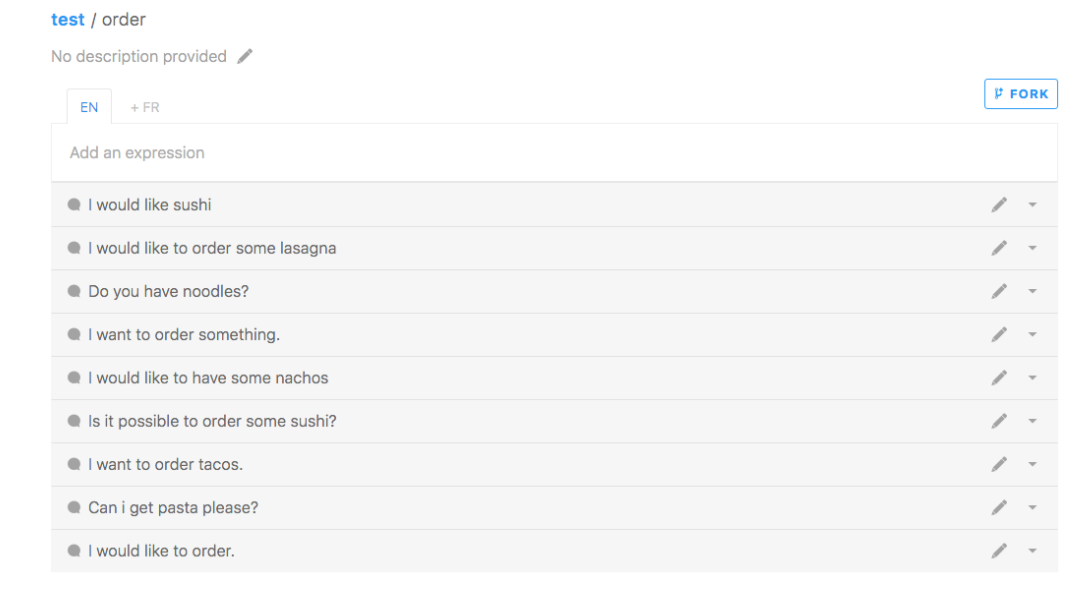
\includegraphics[width = \textwidth]{utterances.png}
	\caption{Liste d'utterances pour l'intent order}
	\label{fig:Liste d'utterances pour l'intent order}
\end{figure}
\vspace{1em}

Pour avoir plus de compréhension de la part de l’utilisateur, on peut mettre en place des entités comme exemple avec « I would like sushi » en mettant sushi dans une catégorie food.
\vspace{1em}

	La dernière étape est le test des utterances qu’on lui a apprises avec un tchat interne. En reprenant l’exemple d’une commande sushi, cela donne un JSON qui contient les informations sur le message.
Voici le test :
\vspace{1em}

\begin{figure}[H]
	\centering
		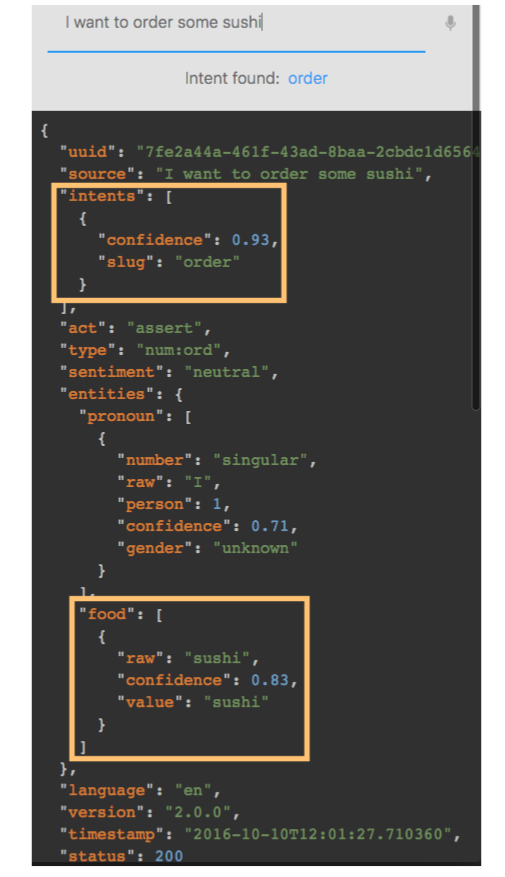
\includegraphics[width = 0.5\textwidth]{test.png}
	\caption{Test de l'intent order}
	\label{fig:Test de l'intent order}
\end{figure}
\vspace{1em}

En entrant I want to ordersome sushi, on a une correspondenceà 93\% avec l’intentorder qui se rapproche le plus avec « I want to ordersomething ».
\vspace{1em}

Il reconnait notamment sushi comme une entité food à 83\%.

\subsubsection{Construire}

Quand tous les intents sont bien paramétrés, il reste à définir un enchaînement des actions pour arriver à une des tâches précises de l’utilisateur.
\vspace{1em}

	En prenant l’exemple du départ d’une commande, on peut se retrouver avec un processus semblable à :
\vspace{1em}

\begin{figure}[H]
	\centering
		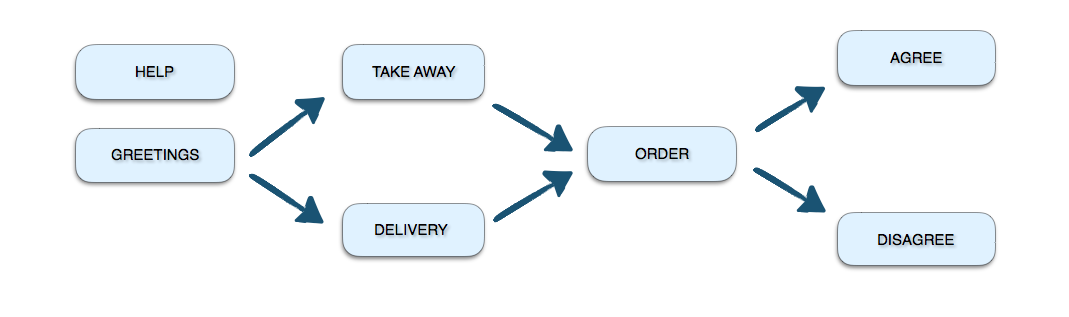
\includegraphics[width = \textwidth]{construire.png}
	\caption{Dialogue flow}
	\label{fig:Dialogue flow}
\end{figure}
\vspace{1em}

Cette partie se fait avec un outil interne mais il peut bien évidemment se faire par la programmation en définissant l’ordre des exécutions et les questions du chatbot à chaque étape. On peut ensuite tester de nouveau  le chatbot.

\subsubsection{Exécuter}

Comme vu dans la partie concept d’un chatbot, il faut mettre « l’outil à disposition » sur un ou plusieurs canaux ;  pour ça, il existe plusieurs librairies qui permettent une connexion vers Messenger, SMS, MAIL, etc.

\subsubsection{Entraîner}

Après le déploiement sur un canal, on peut continuer à le faire évoluer en entrant d’avantage d’intent, d’utterance et de complexification avec des entités. On peut notamment récupérer ou voir les énoncés entrés par les utilisateurs pour perfectionner le chatbot.

\section{Evaluations}

Nous avons diverses méthodes de création d’un chatbot qui sont les plus répandues. Comme nous l’avons dit, le problème reste la compréhension réelle de l’utilisateur par le bot. Elle passe par deux gros problèmes : premièrement par les mots utilisés qui doivent être compris avec une bonne orthographe et deuxièmement par le sens d’une phrase.
\vspace{1em}

Avec le nltk, l’orthographe peut poser problème pour l’analyse sémantique ; 90\% de succès de l’analyse pour l’étiquetage quand il n’y a  aucune faute donc moins s’il y en a.
Pour le sens si l’étiquetage est réussi, alors l’arbre représenté sera bon et ce sera au programme ensuite de faire la compréhension du sens de la phrase même si cela ne sera pas toujours exact.
\vspace{1em}

Avec l’aiml, l’orthographe pose beaucoup de problèmes car elle fait qu’on ne peut rentrer dans aucune catégorie, pour le sens l’aiml est fait pour orienter l’utilisateur autant dans les questions que dans les réponses donc il n’y a aucun problème.
\vspace{1em}

Pour les intents, en écrivant des phrases type, on peut faire quelques erreurs mais se rapprocher le plus possible d’un intent et avec plus d’utterance on réduit les risques. Quant au sens, c’est mieux en proposant à l’utilisateur ces actions possibles et en l’aiguillant dans un domaine plus fermé que le nltk ou l’aiml avec des processus de dialogue.
\vspace{1em}

Un chatbot est avant tout une conversation et ces méthodes la gèrent différemment. Le nltk ne fait que l’analyse de la phrase, il faut ensuite programmer une conversation, un échange, des réponses et une logique. L’aiml quant à lui ne fait que la conversation avec des entrées et des sorties pré-programmées  avec de la logique vue précédemment. Pour finir, l’intent gère tout avec des outils simples et efficaces pour paramétrer un bot.
\vspace{1em}

Un chatbot se veut intelligent dans ses réponses ;  pour le nltk et l’intent tout dépend de l’algo après analyse ou matching avec un intent donc c’est compliqué à évaluer contrairement à l’aiml qui n’en a quasiment aucune. Le machine learning et la base de connaissances sont une part de l’intelligence et elles peuvent être utilisées dans ces méthodes mais le mémoire ne détaille pas ces sujets donc on n’en tiendra pas compte.
\vspace{1em}

\section{Etat de l’art des solutions}

n prenant les critères évoqués dans la partie précédente, on peut facilement enlever l’aiml qui n’offre que très peu de possibilités en termes de programmation et de logique.
Ensuite pour le nltk et les intents, on peut faire de l’algorithme dans les deux méthodes. On pourrait choisir le nltk, si on choisissait de faire un dialogue avec un robot physique, le python étant un langage utilisé pour les programmer.
\vspace{1em}

L’intent semble être la meilleure solution car simple à programmer avec des outils comme celle de la start up recast.ai. Evidemment, il y en d’autres comme IBM, Facebook, Microsoft ou encore Amazon qui s’y mettent beaucoup.
\vspace{1em}

La solution des intents est nouvelle et innovante. Elle évolue beaucoup et colle parfaitement avec l’ère actuelle des différents canaux de discussion. Nous allons nous y intéresser davantage pour savoir si elle permet un paramétrage d’un chatbot intéressant tout en évaluant ses limites avec la partie compréhension du dialogue comme axe principal de notre problématique.
\vspace{1em}

Dans ce dialogue, avec le NLP, la partie NLU est gérée par le moteur de l’outil sélectionné, on ne pourra que choisir les intents pour orienter, les utterances pour augmenter la compréhension et les entities pour plus de choix.
La partie NLU sera programmée et on pourra ajouter une base de connaissances et du machine learning.
\vspace{1em}

L’outil utilisé pour les intents sera LUIS (Language Understanding Intelligent Service) couplé avec Microsoft bot framework pour la partie programmation. Le choix de ces outils m’a été suggéré au cours de mon stage car il s’est déroulé dans une entreprise filiale de Microsoft et donc j’ai eu la chance d’avoir de la documentation, des présentations sur ce domaine et des gens qualifiés.
